\documentclass{article}
\usepackage[T1]{fontenc}
\usepackage[serbian]{babel}
\usepackage[table]{xcolor}
\usepackage[utf8]{inputenc}
\usepackage{graphicx}
\date{\displaydate{date}}

%\title{Seminarski rad iz tehničkog i naučnog pisanja

%\textbf{\Huge{Prednosti i mane učenja na daljinu}}}
%\author{Anja Nenadović, Nikolina Šobić, Maša Kočinac, Marina Stanojlović }
%\date{Novembar 2022}

\begin{document}
\begin{titlepage}
    \begin{center}
        \line(1,0){350}\\
        [0.25in] % 0.25in
        \huge{\bfseries Prednosti i mane učenja na daljinu}\\
        [2mm]
        \line(1,0){350}\\
        [1.5cm]
        \textsc{\LARGE Seminarski rad iz tehničkog i naučnog pisanja}
        \textsc{\\ \Large matematički fakultet univerziteta u beogradu}\\
        [8cm]
        
    \end{center}
    

    \makeatletter
    \raggedleft\Large{\today}
    \makeatother
    
    \begin{flushright}
        \textsc{\large{\underline {autori:}}\\}
        \textit{
        \large Kočinac Maša, masakocinac94@gmail.com\\
        \large Nenadović Anja, anja.nenadovic03@gmail.com\\
        \large Stanojlović Marina, marinastanojlovic02@gmail.com\\
        \large Šobić Nikolina, nikolinasobic@gmail.com\\
        }
    \end{flushright}
    
\end{titlepage}

%\begin{document}

%\maketitle

%\cleardoublepage

\tableofcontents 

\cleardoublepage
\section {Uvod}

\textbf{}

Učenje na daljinu je, u stvari, mnogo starije od učenja putem interneta. Ovakav način učenja postojao je mnogo pre nego što su ljudi znali za računar i internet.

U različitim periodima svog razvoja odvijalo se korišćenjem različitih tehnologija kao što su poštanski sistem, radio i televizija i naposletku internet.

E-učenje je proces u kome nastavnici prezuntuju određeni nastavni sadržaj primenom različitih metoda i oblika rada (strategije) i korišćenjem informaciono-komunikacionih tehnologija i na taj način učenicima obezbeđuju sakupljanje novih znanja. E - učenje je interaktivan ili dvosmeran proces između nastavnika i učenika uz pomoć elektronskih medija pri čemu je naglasak na procesu učenja dok su mediji samo pomoćno sredstvo koje upotpunjuje taj proces.

Istorija učenja na daljinu datira još od 1728. godine, kada je prvi put objavljen poziv za takvu vrstu edukacije. Kejleb Filips, je u časopisu Boston Gazet objavio oglas u kojem traži studente za izučavanje lekcija.
Ajzak Pitmen, engleski učitelj stenografije, godine 1840. godine slao je poštom svojim učenicima kratke odlomke iz Biblije koje je trebalo da prepišu. Učenici bi, nakon što urade zadatak, poštom slali svoje radove učitelju.

Neki od zanimljivih prekretnica u razvoju učenja na daljinu:
\begin{itemize}
    \item 1858. godine – Londonski univerzitet je, pored tradicionalnog učenja, nudio i kurseve na daljinu.
    \item 1996. godine – Djuk univerzitet prvi nudi globalne postdiplomske studije u oblasti menadžmenta, kombinujući onlajn i tradicionalnu nastavu.
    \item 1997. godine - Pojavljuju se alatke za onlajn učenje.
    \item 1998. godine – Nastao je termin e-learning.
    \item -2000. godine – Milijarder Majkl Sejlor donira 100 miliona dolara za stvaranje besplatnog onlajn obrazovanja na kvalitativnom nivou Ajvi lige.
    \item -2001. godine – Razvijen je Moodle, virtuelna obrazovna sredina.
    \item -2003. godine - Počeo je sa radom LINK eLearning system.
    \item - 2005. godine – Skoro 3,2 miliona studenata u SAD odabralo je makar jedan onlajn kurs na univerzitetu.
    \item - 2006. godine – Čak 11.200 programa za koledž u SAD kreirani su tako da u potpunosti mogu da se sprovedu kroz onlajn učenje.
    \item -2009. godine – Youtube kategorija EDU predstavlja na hiljade besplatnih predavanja i Blackboard aplikacija za učenje na daljinu postaje dostupna preko Android platforme.
    \item - 2011. godine – Učenje na daljinu postaje idealno rešenje za studente u Britaniji, kojima je trostruko povećana univerzitetska školarina.
\end{itemize}

\section{Prednosti online učenja}

Da li onlajn ucenje doprinosi ili oduzima od edukacije aktuelna je tema već godinama. Kako među studentima, tako i među profesorima postoji stalna debata o tome koji vid učenja je bolji. Napisano je bezbroj radova na ovu temu u pokušaju da se dođe do zaključka, ali je činjenica da je učenje putem interneta postala neophodna strategija za obavljanje normalnog nastavnog rada u ovom posebnom periodu.U ovom delu bavićemo se prednostima koje onlajn učenje donosi.

Prva prednost koju je vredno spomenuti je da onlajn učenje omogućava više slobode. Ne postoji striktni raspored ili pravilo oblačenja koje se mora poštovati. Studenti mogu da upravljaju svojim vremenom onako kako njima odgovara, bez stresa da li će moći da prisustvuju predavanju uživo.

Materijali sa predavanja su dostupni 24 časa dnevno. Ukoliko nekome treba više vremena za određenu temu, ne postoji pritisak da se gradivo pređe u određenom vremenskom periodu. Svako može raditi odgovarajućom brzinom. Pritom, neki profesori istovremeno objavljuju pisanu formu predavanja kao i video zapise, što daje studentima slobodu izbora o načinu prelaska gradiva. Ako se desi da student ne može da prisustvuje nastavi uživo, imaće materijal na koji može da se osloni pri samostalnom učenju.

Ovakav vid nastave omogućava kvalitetno učestvovanje svih studenata u nastavi. Bilo da je problem u povučenosti osobe ili manjku vremena, teško je da u punoj učionici svako dođe do reči i dobije odgovor na sva pitanja, a da se u isto vreme pređe plan gradiva namenjen za tu nedelju.

Po samoj strukturi, onlajn nastava omogućava interakciju između profesora i studenta, a to se odvija putem različitih vidova internet komunikacije. To je asinhrona komunikacija koja je karakteristična za onlajn učenje. Njene prednosti su jasne i precizne povratne informacije, razmena iskustava kako sa nastavnikom, tako i sa vršnjacima. Pored toga, ovakva komunikacija pruža više vremena za osmišljanje i koncipiranje odgovora, kao i dodatno istraživanje tematike pre pružanja odgovora.

Onlajn nastava poseduje jasnu strukturu i kvalitetnu interakciju. Bez istih, nastava postaje puko iščitavanje materijala kao u knjizi. Postoji bezbroj aplikacija koje profesori mogu iskoristiti za interaktivnost tokom učenja. Mnoga istraživanja (Bawaneh et al., 2010; Rienties et al., 2016) ukazala su da digitalne platforme omogućavaju studentima pristup različitim alatima za učenje, davanje informacija o programu, sadržaju kursa, pomoć instruktora, diskusione table, resurse za učenje bez ograničenja vremena i mesta.

Prilikom realizacije onlajn nastave, razvijaju se digitalne veštine, kako kod profesora, tako i kod studenata. Da bi se realizovala onlajn nastava, potreban je osnovni nivo digitalne pismenosti, koja će uskoro postati neophodna u ovom digitalnom dobu.


\section{Mane online učenja}

Kako živimo u digitalnoj eri, u želji da slikovito objasnimo mane nastave na daljinu, najveći broj primera u nastavku će se odnositi na probleme online nastave. Neki od njih se mogu uopštiti i na ostale vidove nastave na daljinu.

Među najčešćim problemima ili lošim stranama u realizaciji online obrazovanja je nedostatak objekata za sprovođenje online obrazovanja i loše online veštine među samim učiteljima i učenicima. 

Povratne informacije učenika prilično su ograničene.
U tradicionalnoj metodi podučavanja koja uključuje interakciju licem u lice s učenikom u učionici, učitelji i predavači mogu dati trenutnu povratnu informaciju učenicima. Povratna informacija licem u lice ima pozitivniji učinak na učenike, jer poboljšava procese podučavanja i učenja i čini ih lakšim, bogatijim i značajnijim, a ujedno poboljšava i nivo motivacije učenicima.

Učenje na daljinu može dovesti do društvene izolacije. Vrlo je važna društvena interakcija za svakog pojedinca. Ona je ključna za svakog učenika kako bi izgradio svoj karakter i razvio komunikacione veštine.  Društvena izolacija u kombinaciji s nedostatkom komunikativnih veština mogu potencijalno dovesti do nekoliko problema s mentalnim zdravljem kao što su veći nivo stresa i negativne misli.

Proces učenja na daljinu zahtieva visok nivo  samomotivacije i discipliine. Odsutnost samomotivacije i nedisciplina  mogu postati glavna prepreka na putu uspeha učenika. U tradicionalnim učionicama postoje brojni faktori koji mogu stalno gurati učenike prema njihovim ciljevima učenja. Komunikacija licem u lice sa učiteljem, odnosno predavačem i strogi rasporedi rade usklađeno kako bi spriečili učenike da skrenu s puta tokom učenja. U mnogim situacijama, studenti su ostavljeni da se sami snalaze bez da ih iko stalno na to podstiče. Učeniciima, na bilo kom nivou obrazovanja potrebni su spoljašnji faktorii koji će ih pokretati i gurati ka ispunjenju sopstvenih ciljeva, a za nastavu na daljinu ne možemo reći da to uvek pruža.

Poteškoće kada je reč o predstavljanju praktičnih aspekata kursa su, verovatno, najveći problem. Posmatrajmo online nastavu, jedan oblik nastave na daljinu. Iako je predavačima, sigurno teško, na učenicima je, možemo slobodno reći, veći moralni teret. Uzmimo za primer jednog budućeg medicinskog radnika koji pohadja online nastavu (suočeni sa trenutnom pandemijom, nije nam teško to da zamislimo) . Posao kojim će se baviti zahteva visok stepen stručnosti i veštine koji se stiču dugotrajnom praksom, što je otežano ako je kurs pohadjan na daljinu.

Kada je reč o proverama znanja, ovakav vid nastave zahteva medjusobno poverenje izmedju predavača i učenika. Ako se ponovo osvrnemo na online nastavu, shvatamo da je jako teško sprečiti varanje na testovima, ali isto tako, i utvrditi da je bilo varanja. 

Jedna od mana s kojojm se susreću online predavači je ta da je neophodno izdvojiti dosta vremena za sam dizajn i izradu intraktivnih i multimedijalnih sadržaja. Tako da je samo prividna ušteda vremena kada je u pitanju online nastava.

\section{Stavovi mladih o učenju na daljinu}

Pandemija virusa Covid19 je radikalno promenila svakodnevnicu ljudi, a naročito vaspitno-obrazovni sistem velikog broja zemalja sveta, između ostalog i Republike Srbije. U nastavku ćemo pogledati jedno istraživanje stavova mladih o učenju na daljinu.

Predmet ovog istraživanja su opažanja studenata o iskustvu online nastave tokom pandemije Covid19. Cilj istraživanja je da se utvrdi kakav je odnos studenata prema online nastavi u okolnostima pandemije i da li postoje razlike u opažanjima prema polu, nivou studija, godini studiranja, zaposlenosti i boravištu ispitanika. Uzorak je činio 91 student Visoke škole strukovnih studija za obrazovanje vaspitača u Kikindi koji su školske 2020/21. pohađali master i osnovne studije.

Upitnik se sastojao od opšteg dela kojim se prikupljaju osnovni podaci o ispitanicima(pol, nivo i godina studija, zaposlenost i boravište) i skalera od 19 tvrdnji koje se odnose na kvalitet onlajn nastave. Upitnik sadrži tri podskale: Nastavno prisustvo(7 tvrdnji), Socijalno prisustvo(6 tvrdnji) i Kognitivno prisustvo(6 tvrdnji). Ispitanici su označavali stepen slaganja ili neslaganja sa ponuđenim tvrdnjama na petostepenoj skali Likertovog tipa:
\begin{itemize}
    \item 1-"uopšte se ne slažem"
    \item 2-"ne slažem se"
    \item 3-"neodlučan sam"
    \item 4-"slažem se"
    \item 5-"potpuno se slažem"
\end{itemize}

\subsection{Rezultati istraživanja}

Posmatrajući strukturu prema polu, uzorak čini 7 ispitanika i 84 isptitanica. Ova neuravnoteženost uzorka prema polu je očekivana, imajući u vidu da najveći procenat studenata ove visokoškolske ustanove čine osobe ženskog pola.

\parskip=\baselineskip
Tabela 1: Struktura ispitanika prema polu
\begin{center}
\rowcolors{1}{pink}{white}
  \begin{tabular}{ | l | c | r |}
    \hline
    pol & vrednost & procenat \\ \hline
    muški & 7 & 7,7 \\ \hline 
    ženski & 84 & 92,3 \\ \hline
    ukupno & 91 & 100 \\
    \hline
  \end{tabular}
\end{center}
\parskip=\baselineskip

Kada je reč o nivou studija, 64 ispitanika čine studenti osnovnih, a 27 studenti master studija. Prema godini studiranja, 37 ispitanika su na drugoj godini osnovnih studija, 27 ispitanika na trećoj godini osnovnih, a 27 na prvoj godini master studija. Zaposlenih ispitanika je 39, a nezaposlenih 52. Boravište na selu ima 22 ispitanika, a boravište u gradu 69 ispitanika. 

\parskip=\baselineskip

Tabela 2: Da li online nastava može zameniti tradicionalnu nastavu?
\begin{center}
\rowcolors{1}{pink}{white}
  \begin{tabular}{ | l | c |}
    \hline
    Mišljenje & Frekvencija \\ \hline
    da, potpuno & 13  \\ \hline 
    delimično, komhinovanje je najbolje & 27  \\ \hline
    ne, tradicionalno je bolje & 20  \\ \hline
    nisam siguran & 31 \\ \hline
    ukupno &  91 \\
    \hline
  \end{tabular}
\end{center}

Tabela 3: Da li je škola obezbedila ućenicima obuku za korišćenje platofrme/aplikacije koja se koristi za online nastavu?
\begin{center}
\rowcolors{1}{pink}{white}
  \begin{tabular}{ | l | c |}
    \hline
    Obuka & Frekvencija \\ \hline
    da & 53  \\ \hline 
    ne & 34  \\ \hline
    usmeno objašnjenje & 4 \\ \hline
    ukupno &  91 \\
    \hline
  \end{tabular}
\end{center}

Tabela 4: Zadovoljstvo učenika postojećim načinima odvijanja nastave
\begin{center}
\rowcolors{1}{pink}{white}
  \begin{tabular}{ | l | c |}
    \hline
    Nivo zadovoljstva & Frekvencija \\ \hline
    uopšte nisam zadovoljan/na & 17  \\ \hline 
    nisam zadovoljan/na & 13  \\ \hline
    nisam ni zadovoljan/na ni nezadovoljan/na & 33 \\ \hline
    zadovoljan/na sam &  15 \\ \hline
    veoma sam zadovoljan/na & 13 \\ \hline
    ukupno & 91 \\
    \hline
  \end{tabular}
\end{center}

Tabela 5: Šta učenike ometa u izvođenju online nastave?
\begin{center}
\rowcolors{1}{pink}{white}
  \begin{tabular}{ | l | c |}
    \hline
    Smetnje & Frekvencija \\ \hline
    nedostatak interakcije sa profesorima & 30  \\ \hline 
    nedostatak interakcije sa učenicima & 17  \\ \hline
    nedostatak različitih sadržaja & 3 \\ \hline
    monotona nastava & 21 \\ \hline
    nedovoljno poznavanje IKT od strane profesora & 20 \\ \hline
    ukupno & 91 \\
    \hline
  \end{tabular}
\end{center}

Tabela 6: Šta treba da uradi škola i profesori da bi se poboljšao kvalitet online nastave?
\begin{center}
\rowcolors{1}{pink}{white}
  \begin{tabular}{ | l | c |}
    \hline
    Smetnje/prepreke & Frekvencija \\ \hline
    da se u nastavi koriste druge platforme za nastavu & 13  \\ \hline 
    da škola organizuje dodatne obuke za profesore & 9  \\ \hline
    da profesori kažu koje platforme poznaju, pa da se one koriste & 33 \\ \hline
    da se organizuju administratori & 34 \\ \hline
    ukupno & 91 \\
    \hline
  \end{tabular}
\end{center}

Rezultati pokazuju da studenti u proseku imaju negativan odnos prema iskustvu onlajn nastave. Ustanovljeno je da postoje statistički značajne razlike izmedju studenata prema nivou i godini studija.

\subsection{Kratka anketa radjena na studentima Matematičkog fakulteta}

Kako bismo upotpunili naš rad, neophona su bila i mišljenja kolega sa samog fakulteta. U nastavku ćemo pogledati odgovore na kratku anketu koju smo postavile našim kolegama.

\begin{center}
    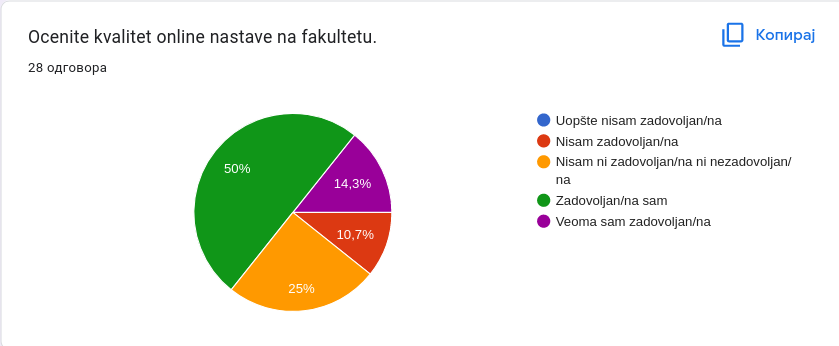
\includegraphics[width=12cm]{1.png}
\end{center}

\begin{center}
    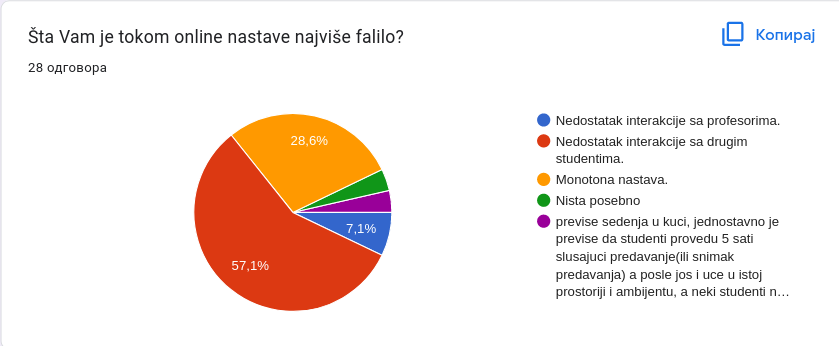
\includegraphics[width=12cm]{2.png}
\end{center}

\begin{center}
    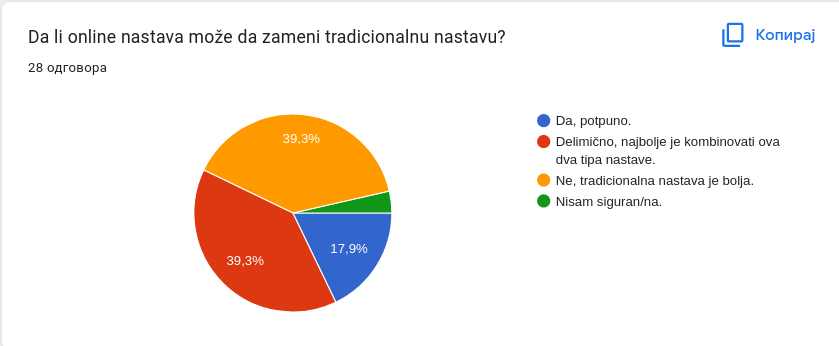
\includegraphics[width=12cm]{3.png}
\end{center}

\newpage

\section{Literatura}
\begin{itemize}
    \item Online nastava u visokom obrazovanju – prednosti, nedostaci i izazovi – Jelena Matijašević, Marko Carić, Sanja Škorić; Univerzitet Privredna akademija, Pravni fakultet za privredu i pravosudje, Novi Sad, Srbija
    \item Prednosti i nedostaci online nastave iz ugla profesora i saradnika – Tatjana Pivac, Milica Pavkov Hrvojević, Lana Zorić; Univerzitet u Novom Sadu, Prirodno-matematički fakultet, Novi Sad, Srbija
    \item Online education in Malaysia: THE GOOD, THE BAD, THE UGLY AND THE WAY FORWARD, Muzaffar Syah Mallow and Syed Saddiq Syed Abdul Rahman
    \item Rezultati-istrazivanje-o-stavovima-mladih-o-onlajn-obrazovanju-u-Srbiji
    \item Opažanja studenata o iskustvu onlajn nastave tokom pandemije Covid-19 - Vasiljevic Danica - Markovic Zagorka
\end{itemize}

\end{document}
